\documentclass{article}

\usepackage{fancyhdr}
\usepackage{extramarks}
\usepackage{amsmath}
\usepackage{hyperref}
\usepackage{amsthm}
\usepackage{amsfonts}
\usepackage{amssymb}
\usepackage{tikz}
\usepackage[plain]{algorithm}
\usepackage{algpseudocode}
\usepackage{diagbox}
\usepackage{gensymb}
\usepackage{comment}
\usepackage{float}
\usepackage{pifont}
\usepackage{graphicx}
\graphicspath{ {./images/}{../}{../../}{../../../}{./} }
\usepackage{bookmark}
\usepackage{multicol}
\setlength{\columnsep}{1cm}
\allowdisplaybreaks

\usetikzlibrary{automata,positioning}

%
% Basic Document Settings
%

\topmargin=-0.45in
\evensidemargin=0in
\oddsidemargin=0in
\textwidth=6.5in
\textheight=9.0in
\headsep=0.25in

\linespread{1.1}

\pagestyle{fancy}
\setlength{\headheight}{22.54448pt}
% \renewcommand{\sectionmark}[1]{
% \markboth{\thesection\quad #1}{}}
\fancyhead{}
\fancyhead[L]{\hmwkAuthorName\ \hmwkAuthorSID\\
\hmwkClass\hmwkClassTime\ (\hmwkClassInstructor): \hmwkTitle}
\fancyhead[C]{}
\fancyhead[R]{\rightmark}
\fancyfoot{}
\fancyfoot[C]{\thepage}

\renewcommand{\sectionmark}[1]{\markright{\thesection.\ #1}}

\renewcommand\headrulewidth{0.4pt}
\renewcommand\footrulewidth{0.4pt}

\setlength\parindent{0pt}

\newcommand{\fakesection}[1]{%
  \par\refstepcounter{section}% Increase section counter
  \sectionmark{#1}% Add section mark (header)
  \addcontentsline{toc}{section}{\protect\numberline{\thesection}#1}% Add section to ToC
  % Add more content here, if needed.
}

%
% Homework Details
%   - Title
%   - Due date
%   - Class
%   - Section/Time
%   - Instructor
%   - Author
%

\newcommand{\hmwkTitle}{Mid-term Report}
\newcommand{\hmwkDoneDate}{\today}
\newcommand{\hmwkClass}{AIST4998/AIST4999}
\newcommand{\hmwkClassTime}{}
\newcommand{\hmwkClassInstructor}{Prof. Wei Meng}
\newcommand{\hmwkClassTitle}{AIST Final Year Project}
\newcommand{\hmwkAuthorName}{YUEN Yu Ching}
\newcommand{\hmwkAuthorSID}{1155143580}

\usepackage{hyperref}
\hypersetup{
    colorlinks=true,
    linkcolor=blue,
    filecolor=magenta,
    citecolor=teal,
    urlcolor=blue,
    pdftitle = {\hmwkClass\hmwkClassTime\ \hmwkTitle},
    pdfauthor = {\hmwkAuthorName \hmwkAuthorSID},
}
\urlstyle{same}

%
% Title Page
%

\title{WEI2202 Mid-Term Report}
\author{YUEN Yu Ching 1155143580}
\date{\today}

\renewcommand{\part}[1]{\textbf{\large Part \Alph{partCounter}}\stepcounter{partCounter}\\}

%
% Various Helper Commands
%

% Useful for algorithms
\newcommand{\alg}[1]{\textsc{\bfseries \footnotesize #1}}

% For derivatives
\newcommand{\deriv}[1]{\frac{\mathrm{d}}{\mathrm{d}x} (#1)}

% For partial derivatives
\newcommand{\pderiv}[2]{\frac{\partial}{\partial #1} (#2)}

% Integral dx
\newcommand{\dx}{\mathrm{d}x}

% Alias for the Solution section header
\newcommand{\solution}{\textbf{\large Solution}}

%Probability
\newcommand{\prob}[1]{\mathrm{P(}\textrm{#1}\mathrm{)}}

% Probability commands: Expectation, Variance, Covariance, Bias
\newcommand{\E}{\mathrm{E}}
\newcommand{\Var}{\mathrm{Var}}
\newcommand{\Cov}{\mathrm{Cov}}
\newcommand{\Bias}{\mathrm{Bias}}
\newcommand{\Or}{\textnormal{ or }}

\begin{document}
\maketitle
\begin{multicols}{2}
\section{Testing Environment}
For this project, we prepared the following hardware for testing:
\begin{itemize}
\item[-]{
\textbf{Raspberry Pi Model 3B+}: The Raspberry Pi Model 3B+ ("Pi" below) is a small single-board computer. It comes with a BCM2837B0 quad-core CPU, which has a 32-bit ARMv8-A architecture. It is capable of Ethernet, WiFi, and Bluetooth networking. We have installed the Raspberry Pi OS on the system, as officially provided and supported by Raspberry Pi \cite{rasppi.os.2022}.\\
Due to its real-world usage as part of IoT systems (as detailed in \cite{9767905}, \cite{8597424}, and \cite{8356449}), we have adopted it to emulate an end node in a IoT network in this project.
\begin{minipage}{0.4\textwidth}\begin{figure}[H]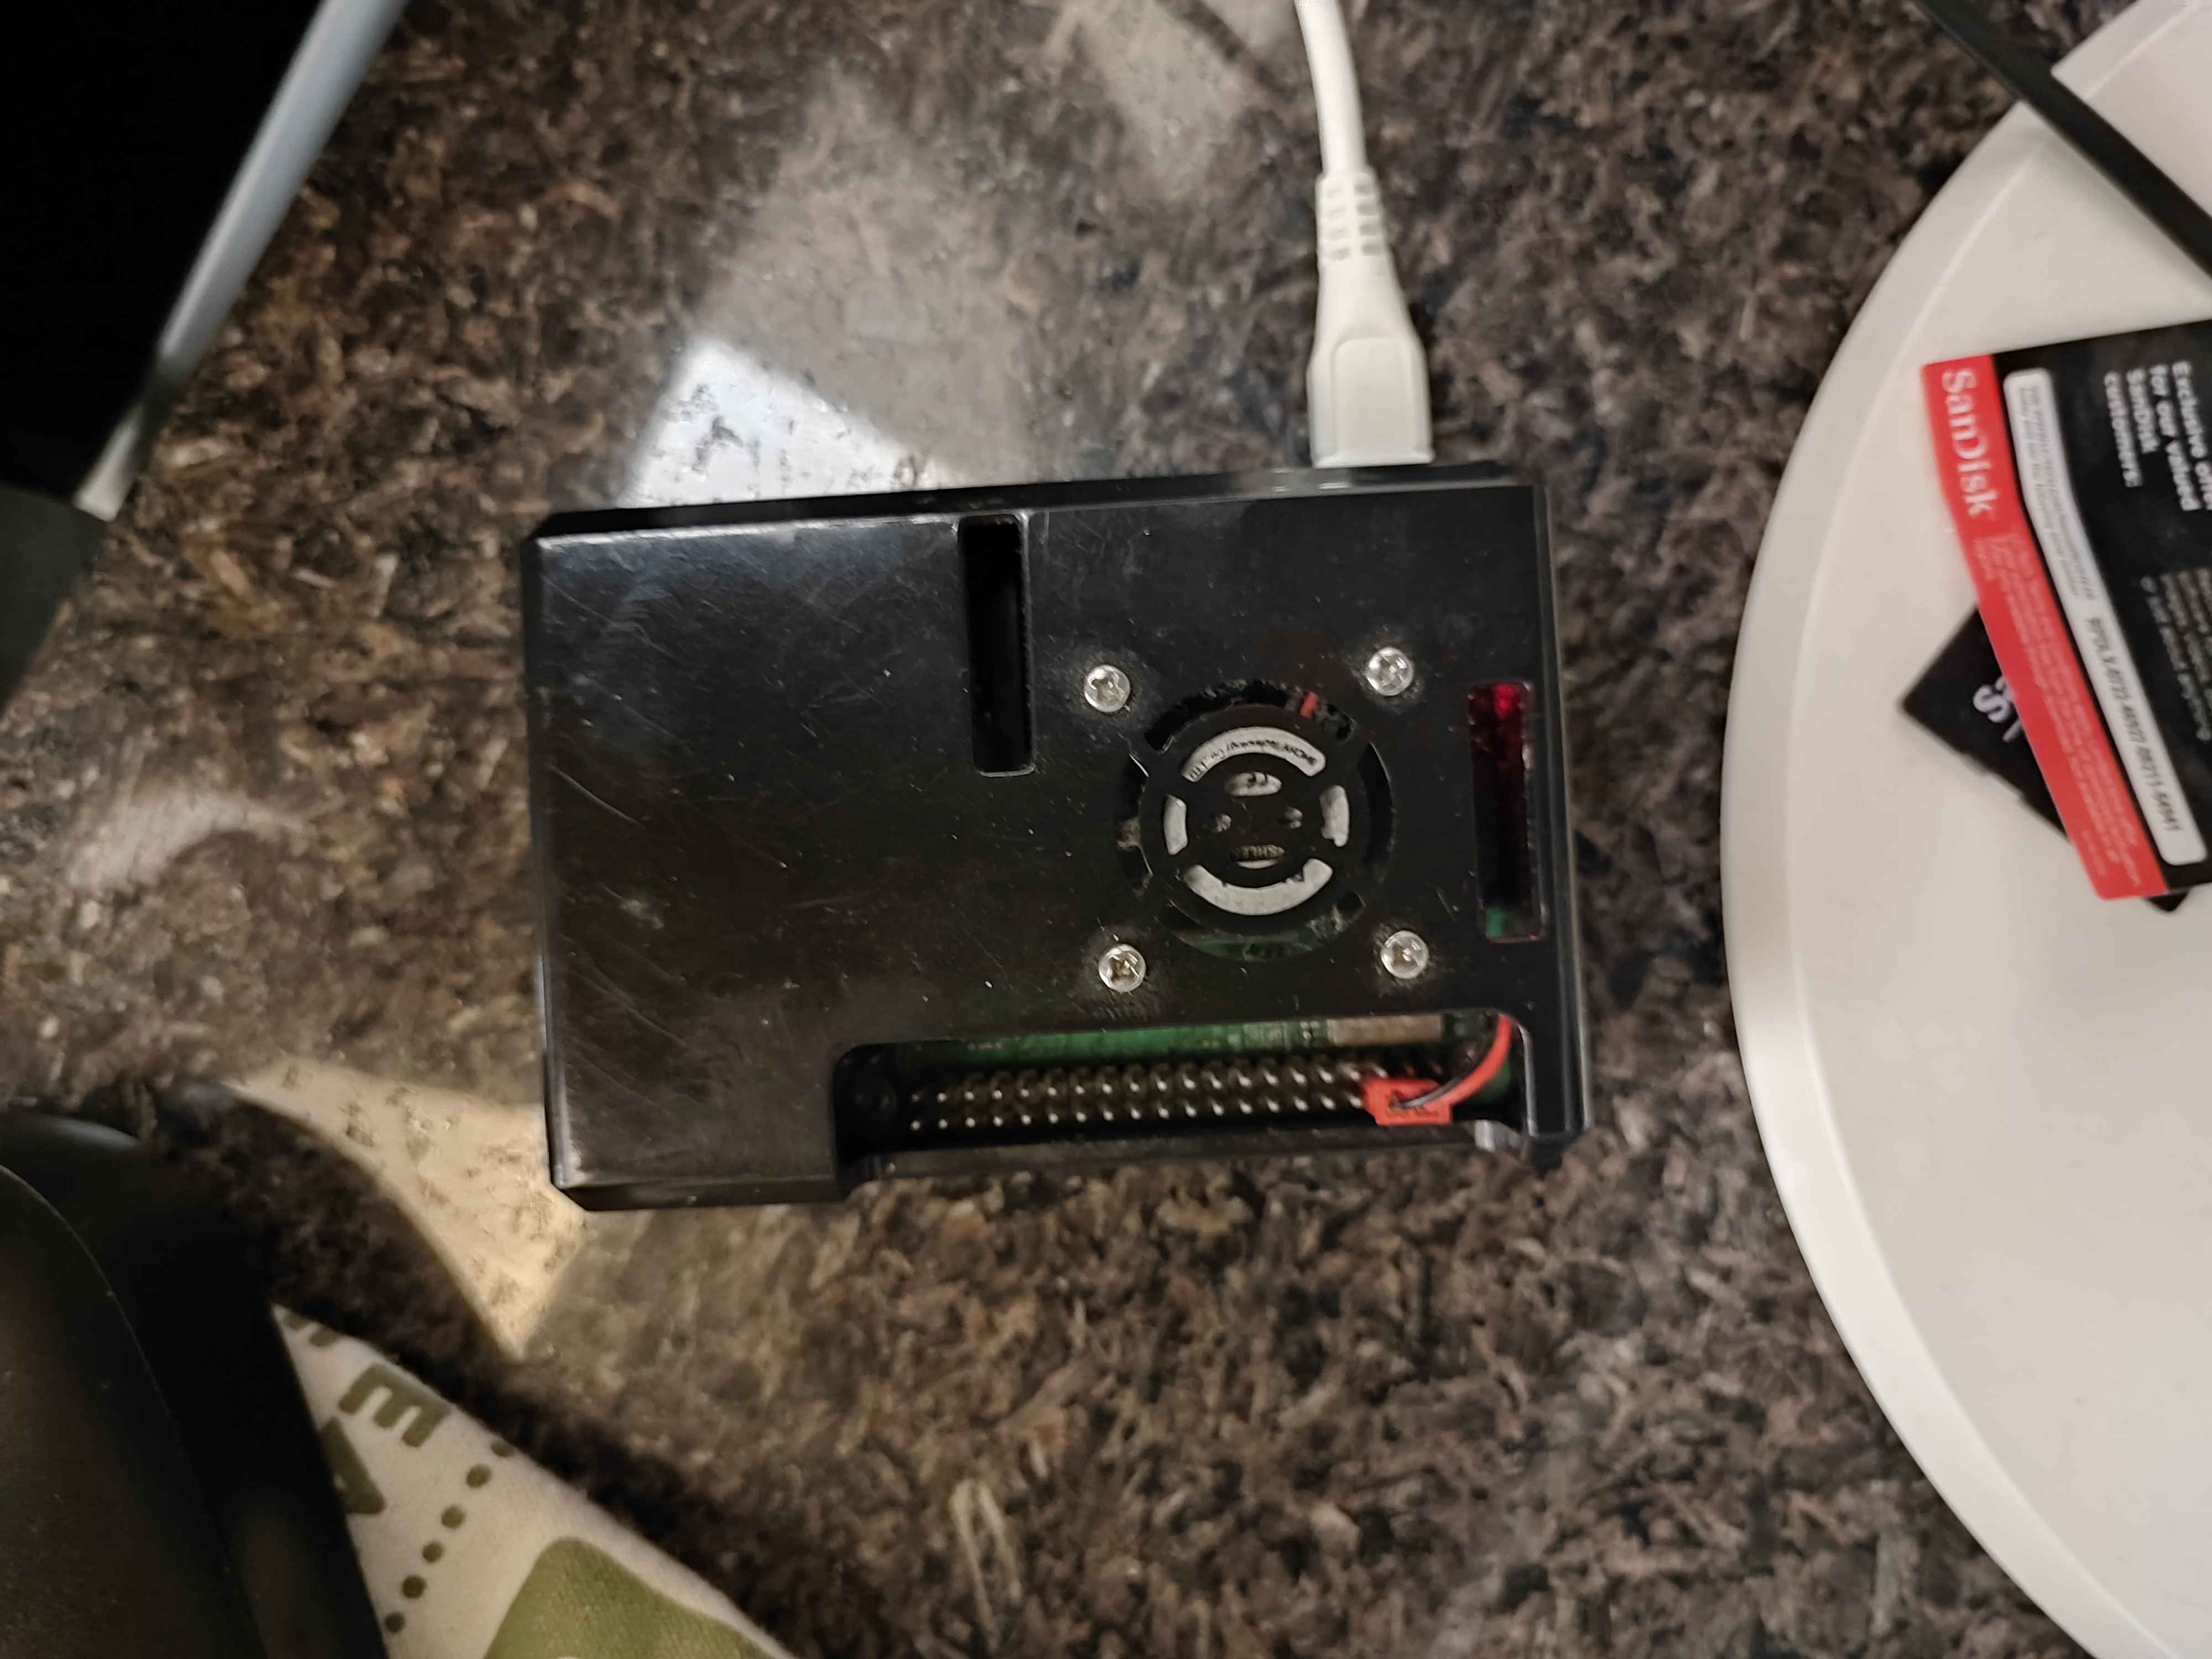
\includegraphics[width=\linewidth]{rasppi}
\caption{Raspberry Pi Model 3B+}
\end{figure}\end{minipage}
}
\item[-]{
\textbf{Mi Gaming Laptop 15.6}: The Mi Gaming Laptop ("Laptop" below) is a relatively high-end laptop. It features a Intel i5 8-core CPU, with NVIDIA GeForce GTX 1660 Ti Mobile; making it suitable for relatively heavy computing work.\\
In this project, we will be using it to emulate a server/gateway serving as an intermediary between the end node and the end user. Due to its popularity in server contexts, Debian GNU/Linux has been installed on this machine.\\
\begin{minipage}{0.4\textwidth}\begin{figure}[H]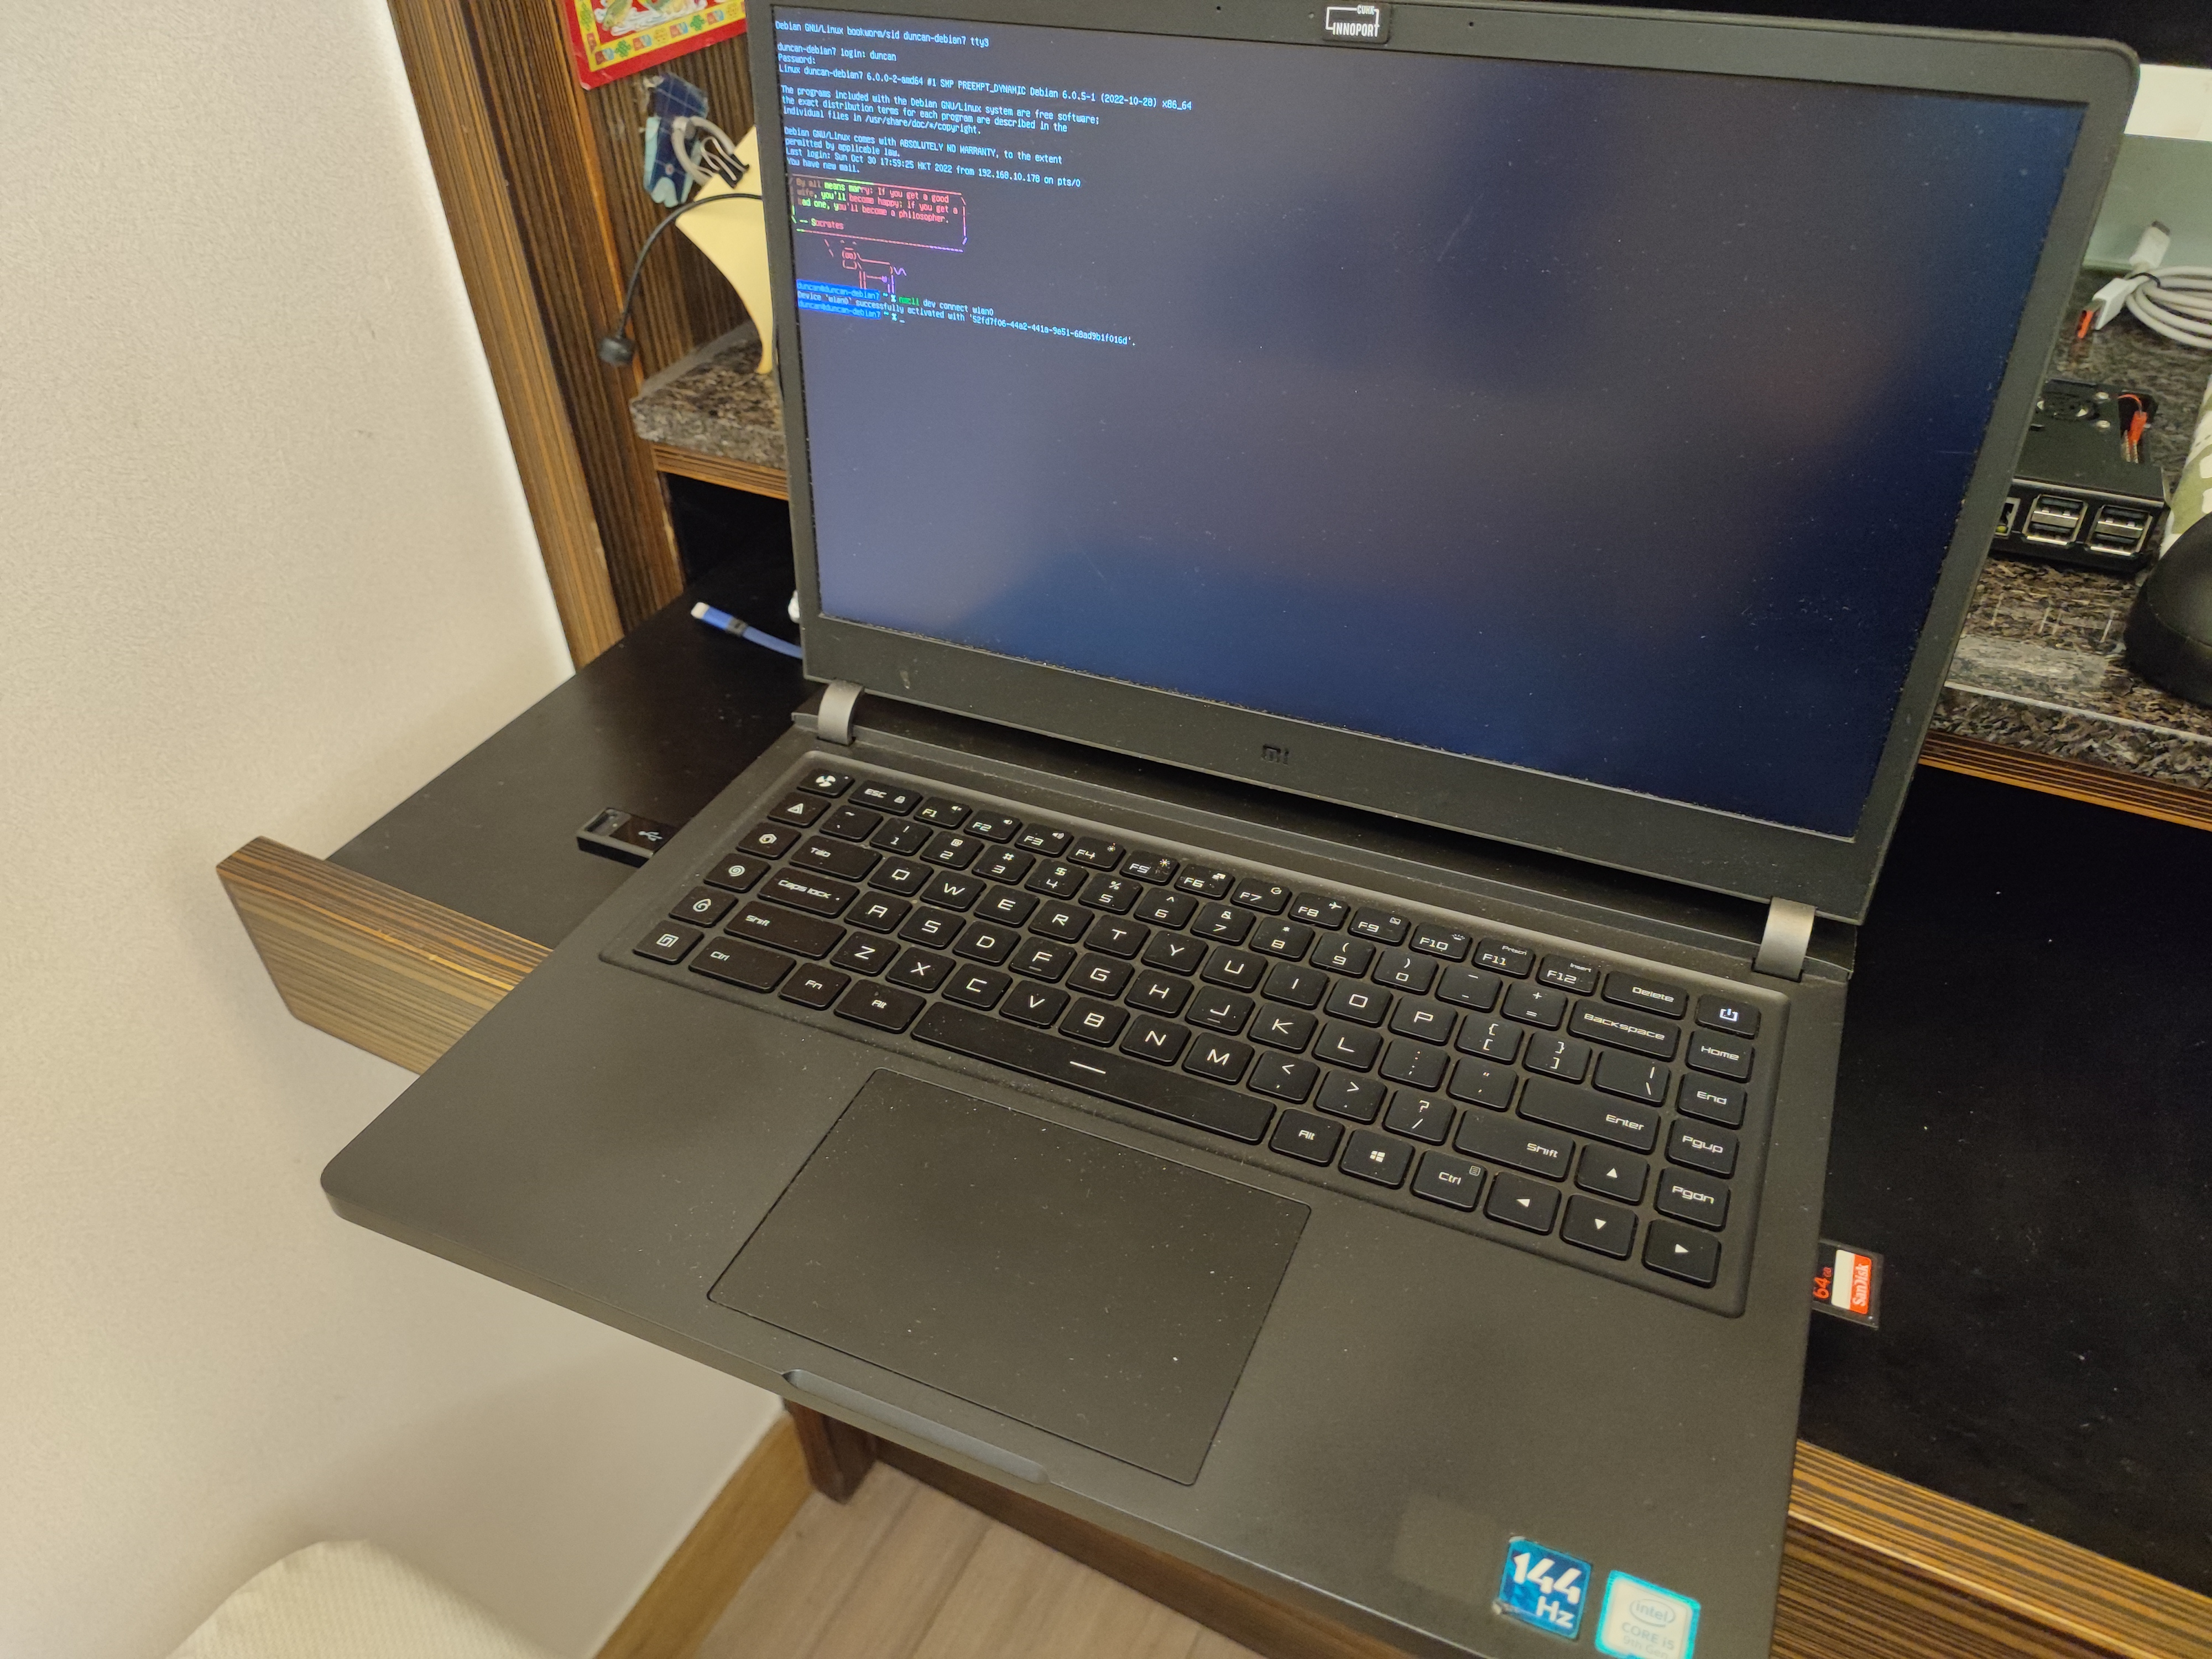
\includegraphics[width=\linewidth]{Laptop}
\caption{Mi Gaming Laptop 15.6}
\end{figure}\end{minipage}
}
\end{itemize}
In addition to the above equipment, we also prepared a small-size sample Internet-of-Things application for testing purposes.
Due to the lack of environmental sensors available, we choose to use the CPU temperature of the Raspberry Pi to act as a pseudorandom statistic for testing purposes.\\
% diag. of structure...
\begin{minipage}{0.4\textwidth}\begin{figure}[H]\includegraphics[width=\linewidth]{WEI2202-system-1.0}
\caption{Structure of the system}
\end{figure}\end{minipage}\\\\
The Pi acts as an end node, which will report its detected CPU temperature to the server every \(5\) seconds via a HTTP POST request. Meanwhile, the Laptop with a server running will receive the request; currently it is configured to print out the received content, with no further action.
\section{Progress}
We have installed Suricata from the Debian official repositories, and successfully ran it on the Laptop for a \(10\)-minute period; during which Suricata executed as expected. The relevant logs can be found here: \href{https://github.com/duncanyuen/WEI2202/tree/main/logs/log-202210312215}{\underline{https://github.com/duncanyuen/WEI2202/tree/}} \href{https://github.com/duncanyuen/WEI2202/tree/main/logs/log-202210312215}{\underline{main/logs/log-202210312215}}
\section{Next Steps}
As outlined in the planning report, we are aiming to finish the IDS within the next month. Our future plans for this period are as follows:
\begin{itemize}
\item[1.]{
Locally compile and run Suricata, with relevant optimizations
}
\item[2.]{
Compile situation-specific rules for Suricata
}
\item[3.]{
Develop an example IoT app over Bluetooth for testing purposes
}
\item[4.]{
(Next phase) Create playbook of attacks
}
\end{itemize}
\end{multicols}

\bibliographystyle{IEEEtran}
\bibliography{3_midterm}

\end{document}

%mail to eeric lo: poster, extention to budget


1. Running RaspPi
2. Running Suricata
3. Detection on Wi-Fi, LAN, Bluetooth
4. Sample IoT application, with Suricata capturing
5. Proof-of-Concept dataset

1. Invalid structure
2. No signal
3. Possible scanning

1. Compile + run, optimizations
1.1 tcmalloc
1.2 runmodes
1.3 tuning considerations
